\documentclass[notes, xcolor=dvipsnames]{beamer}

\usetheme{Berkeley}

\usepackage{inputenc}
\usepackage{graphicx}
\usepackage{amsmath}
\usepackage{amsthm}

\usepackage{subcaption}
\usepackage{multicol}

\title{COMP 513}
\subtitle{Sushmit Sarkar, Peter Sewell, Jade Alglave, Luc Maranget, Derek Williams}

\author{Presented by \\ Akshay Gopalakrishnan}


\begin{document}

    \begin{frame}

        \maketitle

    \end{frame}


    \begin{frame}{Overview}

        \tableofcontents
        
    \end{frame}


    \section{Introduction}

    \begin{frame}{Project Description}


        \begin{center}
            Rolis: A software approach to efficiently replicating multi-core transactions 
        \end{center}

        \begin{itemize}
            \item Proposes a new consensus algorithm to improve throughput. 
            \item Idea is to use multiple threads per leader/follower to process transactions. 
            \item The proposed algorithm also performs well upon failure recovery using watermarks to ensure synchronization when necessary.
        \end{itemize}

    \end{frame}

    \begin{frame}{Choice of Experiments}

        \begin{itemize}
            \item Throughput
            \begin{itemize}
                \item vs Silo - Algorithm is built by modifying Silo.  
                \item vs Calvin - Existing state of the art. 
            \end{itemize}    
            \item Latency - On different batch sizes.           
        \end{itemize}

        
    \end{frame}

    

    \section{Setup}

    \begin{frame}{System Configuration}

        Choice of system

    \end{frame}

    \begin{frame}{How we ran it}

        \begin{itemize}
            \item Security Groups
            \item .... 
            \item Start EC2 instances.
            \item Setup IP addresses via (link to environment setup) guide given by the paper.
            \item ... 
            \item Run $\text{one-click}.\text{sh}$.
        \end{itemize}

    \end{frame}

    \begin{frame}{Differences}

        Differs from original system
        \begin{multicols}{2}
            \begin{itemize}
                \item CPU 
                \item RAM 
                \item NETWORK
                \item OS 
                \item CPU 
                \item RAM
                \item NETWORK
                \item OS 
            \end{itemize}      
        \end{multicols}

    \end{frame}

    \section{Experiments}


    \begin{frame}{Choice}

        \begin{itemize}
            \item Reasons
        \end{itemize}

    \end{frame}

    \begin{frame}{Throughput Rolis vs Silo}
        
        \begin{figure}
            \begin{subfigure}[h]{0.4\textwidth}
                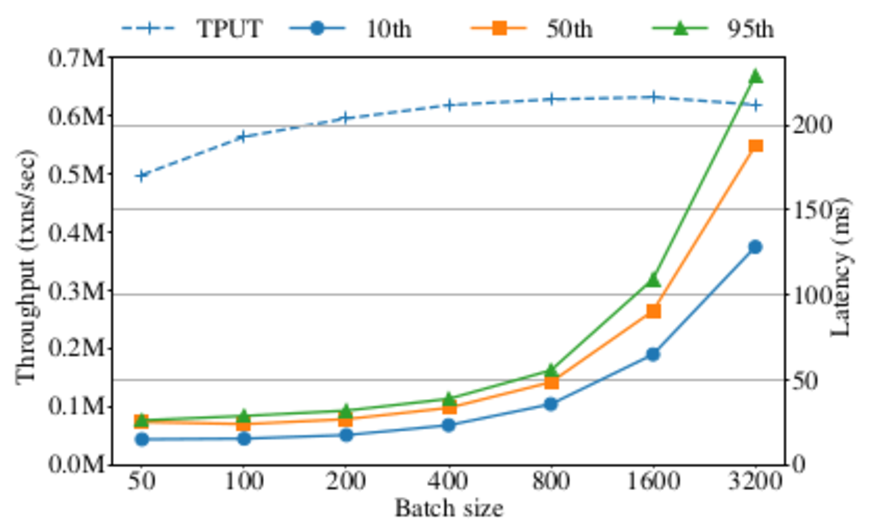
\includegraphics[scale=0.35]{RolisBatch1.pdf}
                \caption{Image A}
            \end{subfigure}
            \hfill
                \begin{subfigure}[h]{0.4\textwidth}
                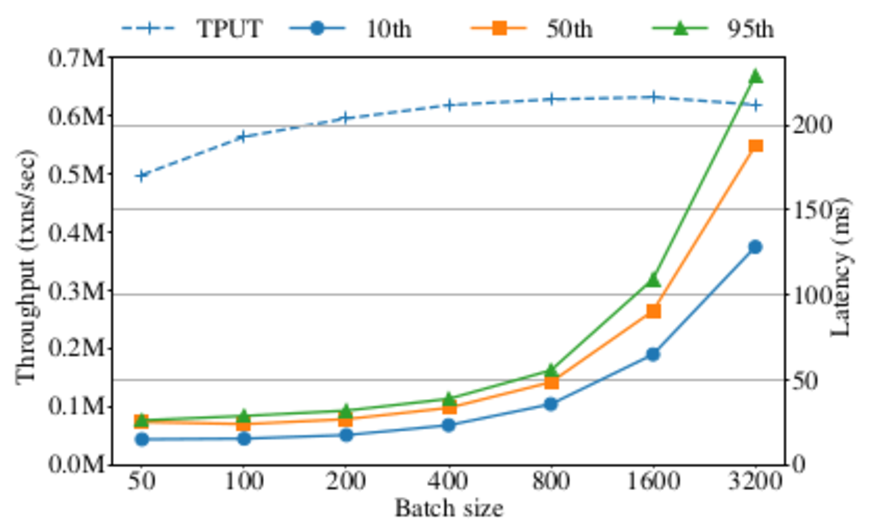
\includegraphics[scale=0.35]{RolisBatch1.pdf}
                \caption{Image B}
            \end{subfigure}%
            \caption{This is a figure with two subfigures}
        \end{figure}

    \end{frame}

    \begin{frame}{Discuss}
        TBD
    \end{frame}


    \begin{frame}{Throughput  Rolis vs Calvin}
        \begin{figure}
            \begin{subfigure}[h]{0.4\linewidth}
                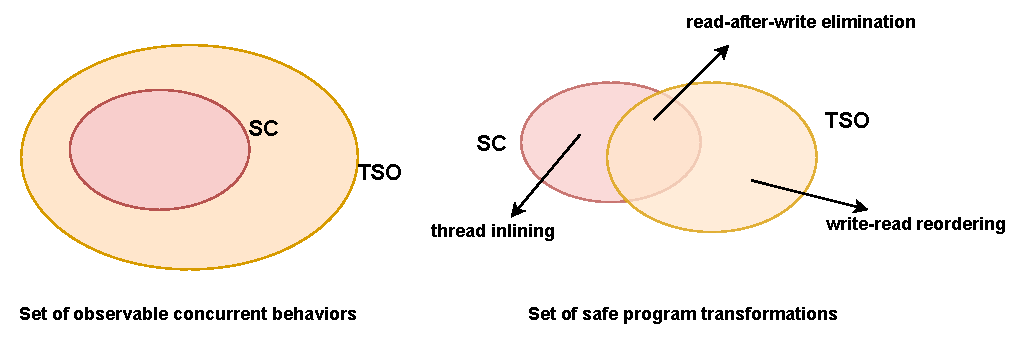
\includegraphics[width=\linewidth]{sample.pdf}
                \caption{Image A}
            \end{subfigure}
                \hfill
                \begin{subfigure}[h]{0.4\linewidth}
                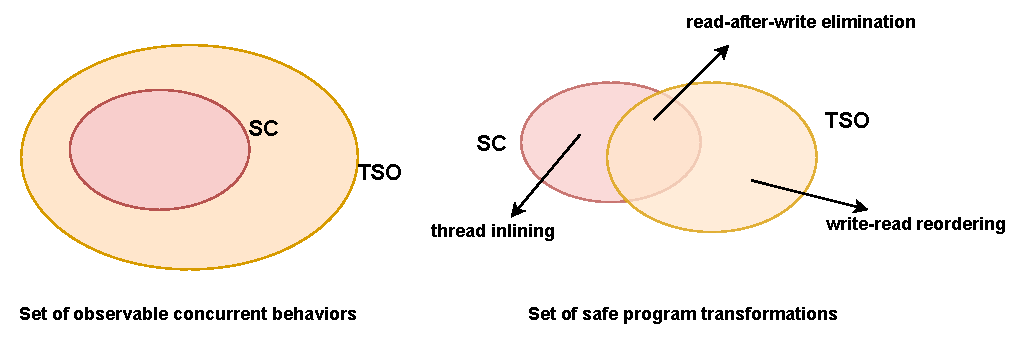
\includegraphics[width=\linewidth]{sample.pdf}
                \caption{Image B}
            \end{subfigure}%
            \caption{This is a figure with two subfigures}
        \end{figure}

    \end{frame}

    \begin{frame}{Discuss}
        TBD
    \end{frame}


    \begin{frame}{Batch}

        \begin{figure}
            \begin{subfigure}[h]{0.4\linewidth}
                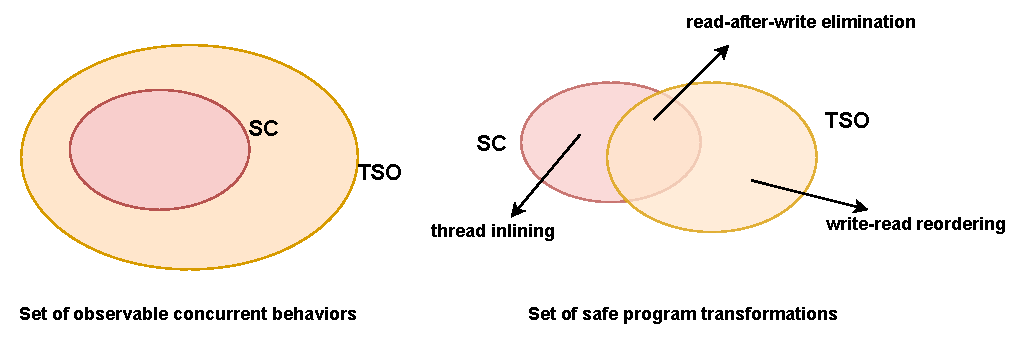
\includegraphics[width=\linewidth]{sample.pdf}
                \caption{Image A}
            \end{subfigure}
                \hfill
                \begin{subfigure}[h]{0.4\linewidth}
                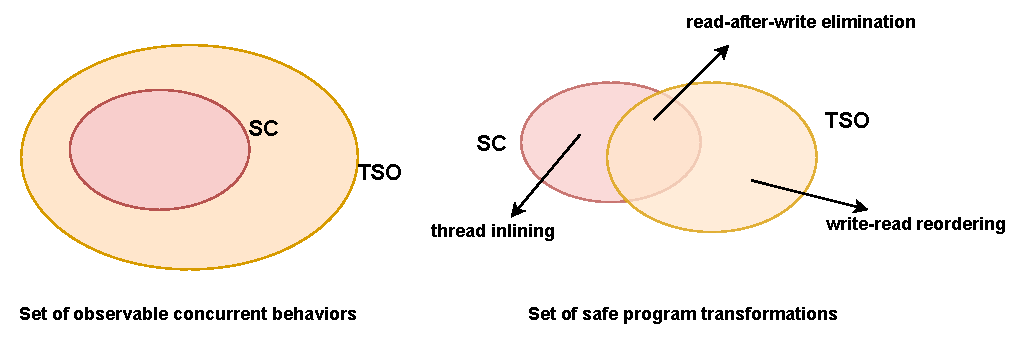
\includegraphics[width=\linewidth]{sample.pdf}
                \caption{Image B}
            \end{subfigure}%
            \caption{This is a figure with two subfigures}
        \end{figure}

    \end{frame}

    \begin{frame}{Discuss}
        TBD
    \end{frame}


    \section{Conclusion}

    \begin{frame}{Thoughts}


    \end{frame}

    \begin{frame} 

    \end{frame}


\end{document}